% =============================================================================
% TEMPLATE ACADÉMICO PARA TRABAJOS EDUCATIVOS
% =============================================================================
% Este template proporciona una estructura completa y profesional para trabajos
% académicos, ensayos, cuestionarios, reportes y otros documentos educativos.
% 
% INSTRUCCIONES DE USO:
% 1. Personalizar las variables de documento en la sección "CONFIGURACIÓN DEL DOCUMENTO"
% 2. Modificar colores en la sección "CONFIGURACIÓN DE COLORES" si es necesario
% 3. Agregar contenido en las secciones correspondientes
% 4. Ejecutar: make build (o pdflatex + biber + pdflatex + pdflatex)
%
% COMPATIBILIDAD LLM:
% - Todas las variables están claramente documentadas
% - Estructura modular para fácil comprensión
% - Comentarios explicativos en cada sección
% =============================================================================

\documentclass[12pt]{article}

% =============================================================================
% CONFIGURACIÓN DE PÁGINA Y GEOMETRÍA
% =============================================================================
% Establece el tamaño de página, márgenes y espaciado general del documento
\usepackage[letterpaper, margin=1in, headheight=0.25in, headsep=0.5in]{geometry}
\setlength{\footskip}{33.5pt} % Espacio para el pie de página

% =============================================================================
% CONFIGURACIÓN DE IDIOMA Y CODIFICACIÓN
% =============================================================================
% Configuración para documentos en español con codificación UTF-8
\usepackage[spanish,es-tabla,es-nodecimaldot]{babel} % Idioma español
\usepackage[utf8]{inputenc}     % Codificación de entrada UTF-8
\usepackage[T1]{fontenc}        % Codificación de fuentes T1
\usepackage{lmodern}            % Fuente Latin Modern mejorada

% =============================================================================
% PAQUETES PARA GRÁFICOS Y TABLAS
% =============================================================================
% Herramientas para inserción de imágenes y creación de tablas profesionales
\usepackage{graphicx}           % Inserción de imágenes
\usepackage{tcolorbox}          % Cajas de texto con color
\usepackage{booktabs}           % Tablas profesionales
\usepackage{tabularray}         % Tablas avanzadas
\usepackage{tabularx}           % Tablas con ancho automático

% =============================================================================
% CONFIGURACIÓN DE FORMATO Y ESPACIADO
% =============================================================================
% Controla el espaciado entre párrafos y otros elementos de formato
\usepackage{parskip}            % Espaciado automático entre párrafos
\usepackage{needspace}          % Control de saltos de página
\usepackage{calc}               % Cálculos matemáticos en LaTeX

% =============================================================================
% PAQUETES PARA COLORES Y DISEÑO VISUAL
% =============================================================================
% Herramientas para personalización visual del documento
\usepackage{xcolor}             % Soporte para colores avanzados
\usepackage{tikz}               % Gráficos vectoriales para headers/footers

% =============================================================================
% CONFIGURACIÓN DE ENCABEZADOS Y PIES DE PÁGINA
% =============================================================================
% Sistema de headers y footers personalizados
\usepackage{fancyhdr}           % Encabezados y pies de página personalizados
\usepackage{lastpage}           % Referencia a la última página

% =============================================================================
% CONFIGURACIÓN DE TÍTULOS Y SECCIONES
% =============================================================================
% Personalización del formato de títulos y secciones
\usepackage{titlesec}           % Personalización de títulos de sección

% =============================================================================
% CONFIGURACIÓN DE ÍNDICES Y TABLA DE CONTENIDOS
% =============================================================================
% Herramientas para generar índices profesionales
\usepackage{tocloft}            % Personalización de tabla de contenidos

% =============================================================================
% CONFIGURACIÓN MATEMÁTICA
% =============================================================================
% Soporte para fórmulas y expresiones matemáticas
\usepackage{amsmath}            % Entorno matemático avanzado

% =============================================================================
% CONFIGURACIÓN DE BIBLIOGRAFÍA
% =============================================================================
% Sistema de referencias bibliográficas con Biber/BibLaTeX
\usepackage[backend=biber, style=apa, sortcites, url=true, autocite=superscript]{biblatex}
\usepackage{csquotes}           % Manejo de citas y comillas

% =============================================================================
% CONFIGURACIÓN DE HIPERVÍNCULOS
% =============================================================================
% Enlaces internos y externos en el documento
\usepackage{hyperref}           % Hipervínculos (debe cargarse al final)

% =============================================================================
% CONFIGURACIÓN DE COLORES DEL TEMPLATE
% =============================================================================
% Paleta de colores principal del documento. Modifica estos valores para
% personalizar la apariencia visual del template.

% Colores primarios (usados en títulos y elementos principales)
\definecolor{primaryColor}{RGB}{124, 10, 2}        % Rojo oscuro principal
\definecolor{secondaryColor}{RGB}{240, 89, 65}     % Rojo medio secundario  
\definecolor{accentColor}{RGB}{239, 167, 0}        % Naranja para acentos

% Colores funcionales
\definecolor{linkColor}{RGB}{239, 167, 0}          % Color para hipervínculos
\definecolor{headerTextColor}{RGB}{255, 255, 255}  % Texto en encabezados
\definecolor{bodyTextColor}{RGB}{0, 0, 0}          % Texto principal del documento

% =============================================================================
% CONFIGURACIÓN DE FORMATO DE TÍTULOS
% =============================================================================
% Personalización visual de secciones, subsecciones y subsubsecciones

% Formato para secciones principales
\titleformat{\section}
    {\color{primaryColor}\Large\bfseries}                    % Estilo del texto
    {\fcolorbox{primaryColor}{primaryColor}{\color{headerTextColor}\thesection}} % Número de sección
    {1em}                                                     % Separación
    {}                                                        % Código antes del título
    [{\titlerule[0.5ex]}]                                    % Línea debajo del título

% Formato para subsecciones
\titleformat{\subsection}
    {\color{primaryColor}\large}                             % Estilo del texto
    {\bfseries\color{primaryColor}\thesubsection}            % Número de subsección
    {1em}                                                     % Separación
    {}                                                        % Código antes del título

% Formato para subsubsecciones
\titleformat{\subsubsection}
    {\color{primaryColor}}                                   % Estilo del texto
    {\bfseries\color{primaryColor}\thesubsubsection}         % Número de subsubsección
    {1em}                                                     % Separación
    {}                                                        % Código antes del título

% =============================================================================
% CONFIGURACIÓN DE ENCABEZADOS Y PIES DE PÁGINA
% =============================================================================
% Sistema personalizado de headers y footers con elementos gráficos

% Eliminar líneas por defecto de fancyhdr
\renewcommand{\headrulewidth}{0pt}
\renewcommand{\footrulewidth}{0pt}

\renewcommand{\arraystretch}{1.5} % Más espacio entre filas de tablas

% Comando para crear caja decorativa en el encabezado
\newcommand{\createHeaderBox}{
    \begin{tikzpicture}[overlay, remember picture, x=1in, y=1in, shift=(current page.north west)]
        \fill[primaryColor] (1,-0.25) rectangle (\headerBoxWidth,-0.5);
        \draw[secondaryColor, ultra thick] (0.25,-0.5) -- (6,-0.5);
    \end{tikzpicture}
}

% Comando para el logo en el pie de página
\newcommand{\createFooterLogo}{
    \color{secondaryColor}\textbf{PUCMM}
}

% Configuración de headers y footers
\fancyhead{}                    % Limpiar encabezados
\fancyfoot{}                    % Limpiar pies de página
\fancyfoot[R]{\createFooterLogo}                              % Logo en pie derecho
\fancyhead[L]{\createHeaderBox\color{headerTextColor}\documentShortTitle} % Título en encabezado izquierdo
\fancyhead[R]{\color{bodyTextColor}Pág.\ \thepage\ -~\pageref{LastPage}} % Paginación en encabezado derecho

% =============================================================================
% CONFIGURACIÓN DE TABLA DE CONTENIDOS
% =============================================================================
% Personalización del índice con puntillismo y espaciado profesional

\renewcommand{\cftsecleader}{\cftdotfill{\cftdotsep}}      % Puntillismo para secciones
\renewcommand{\cftsubsecleader}{\cftdotfill{\cftdotsep}}   % Puntillismo para subsecciones
\setlength{\cftbeforesecskip}{0.5em}                       % Espacio antes de secciones
\setlength{\cftbeforesubsecskip}{0.2em}                    % Espacio antes de subsecciones

% =============================================================================
% CONFIGURACIÓN DEL DOCUMENTO - PERSONALIZAR AQUÍ
% =============================================================================
% Variables principales del documento. Modifica estos valores para personalizar
% tu trabajo académico.

% Información institucional
\newcommand{\universityName}{Pontificia Universidad Católica Madre y Maestra}
\newcommand{\departmentName}{Escuela de Ingeniería en Computación y Telecomunicaciones}     % Ej: Escuela de Ingeniería
\newcommand{\facultyName}{Facultad de Ciencias e Ingeniería}         % Ej: Facultad de Ciencias e Ingeniería

% Información del documento
\newcommand{\documentMainTitle}{Evaluación comparativa de algoritmos de reconocimiento facial en la identificación de características demográficas}     % Título completo
\newcommand{\documentShortTitle}{Evaluación de Algoritmos}                      % Título para headers (máx 20 caracteres)

% Información del curso
\newcommand{\courseName}{Metodología de la Investigación}               % Ej: Metodología de la Investigación
\newcommand{\courseCode}{CSTI-1890-4341}               % Ej: CSTI-1890-4341

% Información del estudiante (mantener datos reales)
\newcommand{\studentName}{Cristian de la Hoz}
\newcommand{\studentId}{(1014-9779)}
\newcommand{\secondStudentName}{Jean Carlos Pérez Ortega}
\newcommand{\secondStudentId}{(1014-8917)}
\newcommand{\thirdStudentName}{Randy Alexander Germosén Ureña}
\newcommand{\thirdStudentId}{(1013-4707)}

% Información del instructor
\newcommand{\instructorName}{Arlene Estévez}        % Ej: Prof. Juan Pérez

% Fechas
\newcommand{\submissionDate}{Julio de 2025}                 % Ej: Enero de 2025
\newcommand{\shortDate}{21/07/2025}                      % Ej: 15/01/2025

% Información del logo institucional
\newcommand{\institutionalLogo}{assets/Logo PUCMM (Color).png}    % Ruta al logo de la institución

% =============================================================================
% GENERACIÓN AUTOMÁTICA DE ARCHIVO BIBLIOGRÁFICO
% =============================================================================
% Cargar archivo de bibliografía
\addbibresource{biblio.bib}

% =============================================================================
% CONFIGURACIÓN DE HIPERVÍNCULOS
% =============================================================================
% Personalización de enlaces internos y externos del documento
\hypersetup{
    linktoc=page,                    % Enlaces en números de página del índice
    colorlinks=true,                 % Colorear enlaces en lugar de cajas
    allcolors=linkColor,             % Color uniforme para todos los enlaces
    pdftitle=\documentMainTitle      % Título en metadatos del PDF
}

% =============================================================================
% CÁLCULO AUTOMÁTICO DE DIMENSIONES
% =============================================================================
% Variables calculadas automáticamente para elementos gráficos
\newlength{\headerBoxWidth}
\AtBeginDocument{
    \setlength{\headerBoxWidth}{\widthof{\documentShortTitle}+1.11in}
}

% =============================================================================
% INICIO DEL DOCUMENTO
% =============================================================================
\begin{document}

% =============================================================================
% PÁGINA DE TÍTULO
% =============================================================================
% Portada profesional del documento generada automáticamente
% =============================================================================
% PÁGINA DE TÍTULO PROFESIONAL
% =============================================================================
% Este archivo genera automáticamente una portada profesional usando las
% variables definidas en el documento principal.

\begin{titlepage}
    \thispagestyle{empty} % Sin numeración en la página de título
    \begin{center}
        
        % Logo institucional
        \includegraphics[width=1.5in]{\institutionalLogo}
        \vspace{0.1in}

        % Líneas decorativas debajo del logo
        \noindent\rule{\textwidth}{0.4pt}
        \noindent\rule{\textwidth}{7pt}
        \vspace{0.1in}

        % Nombre de la universidad
        {\Huge\bfseries \universityName}
        \vspace{0.1in}

        % Información del departamento y facultad
        {\Large\bfseries \departmentName}
        
        {\large\bfseries \facultyName}
        \vspace{0.1in}

        % Título principal del documento en caja colorida
        \begin{tcolorbox}[
            sharp corners,
            boxrule=0pt, 
            colframe=secondaryColor, 
            colback=primaryColor, 
            coltext=headerTextColor, 
            width=1.2\textwidth, 
            center, 
            halign=center
        ]
            \Huge\bfseries \documentMainTitle
        \end{tcolorbox}
        \vspace{0.1in}

        % Información del curso
        {\large\bfseries \courseName}
        
        {\bfseries \courseCode}
        \vspace{0.1in}

        \vfill

        % Información de los estudiantes
        {\large\bfseries \studentName}
        
        {\small\bfseries \studentId}

        {\large\bfseries \secondStudentName}

        {\small\bfseries \secondStudentId}

        {\large\bfseries \thirdStudentName}

        {\small\bfseries \thirdStudentId}

        \vfill
        \vspace{0.1in}

        % Información del instructor
        {\large\bfseries Prof. \instructorName}
        \vspace{0.1in}

        % Fecha de entrega
        \bfseries \submissionDate
        
    \end{center}
\end{titlepage}


% =============================================================================
% TABLA DE CONTENIDOS
% =============================================================================
% Índice automático del documento
\newpage
\pagenumbering{Roman}               % Numeración romana para páginas preliminares
\tableofcontents
\listoffigures
\listoftables
\newpage

% =============================================================================
% CONTENIDO PRINCIPAL DEL DOCUMENTO
% =============================================================================
% Aquí comienza el contenido académico principal
\pagenumbering{arabic}              % Numeración arábiga para contenido principal
\pagestyle{fancy}                   % Activar encabezados y pies de página personalizados

% -----------------------------------------------------------------------------
% SECCIÓN: Resumen y Abstract
% -----------------------------------------------------------------------------
% Presenta el propósito y contexto del trabajo académico
\section{Resumen}

En este estudio se evalúa el rendimiento de diferentes algoritmos de reconocimiento facial en la predicción de características demográficas como la edad, el sexo y la raza, utilizando el conjuntos de datos UTKFace. Se emplearon modelos preentrenados de OpenCV (basados en Caffe), DLib y FaceNet, integrados con clasificadores SVM (Máquina de Vectores de Soporte) para tareas de clasificación multiclase. La métrica principal utilizada fue el F1-score macro, aplicada sobre clases de edad personalizadas y categorías balanceadas de sexo y raza. Los resultados muestran que FaceNet obtiene los mejores desempeños en la clasificación por raza (F1 > 0.87), DLib presenta buena precisión en sexo, mientras que OpenCV muestra limitaciones importantes en la estimación de edad. Se concluye que el tipo de arquitectura y el pre entrenamiento afectan significativamente el rendimiento por tarea. Estos hallazgos son relevantes para aplicaciones sensibles al sesgo demográfico y sugieren líneas de trabajo futuro orientadas al entrenamiento personalizado y al análisis de equidad algorítmica.

\textbf{Palabras clave:} Reconocimiento facial, F1-score, UTKFace, OpenCV, DLib, FaceNet

\section{abstract}
This study evaluates the performance of different facial recognition algorithms in predicting demographic traits such as age, gender, and race using the UTKFace dataset. Pretrained models from OpenCV (Caffe-based), DLib, and FaceNet were used, integrated with SVM (Support Vector Machine) classifiers for multiclass classification tasks. The main evaluation metric was the macro F1-score, applied to customized age ranges and balanced gender and race categories. Results show that FaceNet achieves the best performance in race classification (F1 > 0.87), DLib performs well in gender prediction, while OpenCV reveals significant limitations in age estimation. It is concluded that model architecture and pretraining have a strong impact on task-specific performance. These findings are relevant for applications sensitive to demographic bias and suggest future work focused on custom training and algorithmic fairness assessment.

\textbf{Keywords:} Facial recognition, F1-score, UTKFace, OpenCV, DLib, FaceNet


% -----------------------------------------------------------------------------
% SECCIÓN: INTRODUCCIÓN
% -----------------------------------------------------------------------------
\newpage
\section{Introducción}
Este estudio tiene como objetivo comparar el desempeño de distintos algoritmos de reconocimiento facial en la predicción de atributos demográficos, específicamente la edad, el sexo y la raza. Estas tareas representan un desafío en entornos reales debido a la variabilidad en condiciones de iluminación, expresiones faciales, y diversidad étnica. Como punto de partida, se realizó una revisión general sobre el campo del reconocimiento facial, identificando herramientas ampliamente utilizadas en la industria, entre ellas: OpenCV, DLib y FaceNet. Estas bibliotecas proporcionan modelos pre entrenados y funcionalidades de extracción de características que permiten abordar tareas de clasificación demográfica desde distintos enfoques técnicos. La presente investigación se fundamenta en principios del aprendizaje automático supervisado, específicamente en tareas de clasificación multiclase aplicadas al reconocimiento facial. El objetivo es predecir atributos demográficos como edad, sexo y raza a partir de imágenes faciales, una tarea relevante en diversos dominios como seguridad, análisis de audiencia y personalización de servicios.
% -----------------------------------------------------------------------------
Para evaluar el desempeño de los modelos se emplea la métrica F1-score macro, que permite valorar el equilibrio entre precisión y exhaustividad en contextos donde las clases pueden estar desbalanceadas. Esta métrica es especialmente útil cuando cada clase debe tener el mismo peso en la evaluación, independientemente de su frecuencia.

\subsection{Modelos utilizados}

\begin{itemize}
  \item \textbf{OpenCV} (Caffe-based): Utiliza redes convolucionales entrenadas previamente en un conjunto cerrado de rangos de edad y sexo. Es accesible y rápido, aunque limitado en precisión, especialmente para edades intermedias o extremas etarias.
  \item \textbf{DLib}: Biblioteca que proporciona detección y alineamiento facial, junto con vectores de características embebidas. Sus descriptores pueden ser usados como entrada a clasificadores externos, como SVM, lo que permite entrenar modelos personalizados para predicción de edad, sexo o raza.
  \item \textbf{FaceNet}: Modelo profundo basado en redes neuronales convolucionales con arquitectura Inception, entrenado con la función de pérdida triplet loss. Extrae vectores de alta dimensionalidad que representan rasgos faciales, y al igual que DLib, permite su uso como entrada para clasificadores multiclase.
\end{itemize}

Este estudio es relevante porque permite evaluar comparativamente el desempeño de tres modelos de reconocimiento facial ampliamente utilizados: los proporcionados por las librerías OpenCV, DLib y FaceNet. A través de su aplicación en tareas de predicción de atributos demográficos como edad, sexo y raza, se busca identificar fortalezas y limitaciones en contextos prácticos.

Evaluar modelos pre entrenados bajo un enfoque experimental riguroso no solo permite identificar cuál ofrece mayor precisión global, sino también analizar qué tan bien se comportan en grupos demográficos diversos. Esta información es clave para el diseño de sistemas justos, confiables y alineados con principios de equidad algorítmica.
% ----------------------------------------------------------------------------

% Subsección de ejemplo
\section{Desarrollo}
\subsection{Metodología}
El presente estudio adopta un enfoque cuantitativo y comparativo para evaluar el rendimiento de tres algoritmos de reconocimiento facial OpenCV, DLib y FaceNet en la predicción de atributos demográficos: edad, sexo y raza. Se utilizó UTKFace como dataset, el cual contiene miles de imágenes etiquetadas con metadatos demográficos relevantes.

El experimento consiste en aplicar los modelos pre entrenados disponibles en cada librería sobre subconjuntos estratificados de imágenes, registrando las predicciones generadas y evaluando la precisión de estas mediante la métrica F1-score macro, que permite valorar el rendimiento global en clasificaciones multiclase con clases desbalanceadas.

\subsection{Hipótesis}
\begin{enumerate}
  \item Existen diferencias estadísticamente significativas (p < 0.05, con una diferencia mínima del 5\% en el F1-score), en la capacidad de los algoritmos de reconocimiento facial OpenCV, DLib y FaceNet para identificar características demográficas (rango de edad, sexo y raza) en imágenes faciales, utilizando datos reales obtenidos del dataset UTKFace.

  \item Se espera que, en función de sus características técnicas y enfoques de detección, OpenCV obtenga mejores resultados en la identificación de rangos de edad, alcanzando un F1-score superior al 85\%; que DLib sobresalga en la identificación de sexo, con un nivel de desempeño superior al 90\%; y que FaceNet logre un rendimiento destacado en la clasificación de raza, con una capacidad de clasificación superior al 80\%.
\end{enumerate}

\subsection{Variables}
Basado en la hipótesis planteada, se identifican las siguientes variables:

\begin{itemize}
  \item \textbf{Variable dependiente}: Precisión del algoritmo (F1-score de predicciones correctas).
  \item \textbf{Variables independientes}:
        \begin{itemize}
          \item Raza: caucásico, afrodescendiente, asiático, latino.
          \item Sexo: masculino, femenino.
          \item Rango de edad: 18-23, 23-35, 35-45, 45-55.
        \end{itemize}
  \item \textbf{Variables a controlar}:
        \begin{itemize}
          \item Iluminación (medida en luxes).
          \item Resolución de imagen (píxeles).
          \item Orientación del rostro (grados).
          \item Calidad del sensor (megapíxeles).
        \end{itemize}
\end{itemize}

\subsection{Estrategia del muestreo}

Se empleó un muestreo estratificado, asegurando una representación proporcional de todas las categorías demográficas en cada conjunto de imágenes. Esta técnica se justifica por:

\begin{itemize}
  \item Representatividad: Asegura una representación proporcional de todas las categorías de raza, edad y sexo, reduciendo sesgos en la evaluación de algoritmos (\textbf{OpenCV}, \textbf{DLib}, \textbf{FaceNet}).
  \item Equilibrio entre conjuntos: Compensa distribuciones desiguales.
  \item Validez estadística: Facilita el análisis comparativo de F1-scores entre algoritmos, mejorando la generalización de los resultados.
\end{itemize}

\subsection{Materiales y Métodos}

El conjunto de datos \textbf{UTKFace} es un dataset público ampliamente utilizado en investigaciones de reconocimiento facial con enfoque demográfico. Contiene más de 20,000 imágenes faciales etiquetadas con edad, sexo y raza, cubriendo un rango de edades desde 0 hasta 116 años. Las imágenes fueron recolectadas en condiciones no controladas y presentan variaciones significativas en términos de expresión facial, iluminación, pose y calidad.

Cada archivo de imagen en \texttt{UTKFace} sigue un formato de nombre estructurado:\newline
\texttt{[edad]\_[sexo]\_[raza]\_[timestamp].jpg\_chip.jpg}, donde:

\begin{itemize}
  \item Edad: número entero (por ejemplo, 23 indica 23 años).
  \item Sexo: 0 = masculino, 1 = femenino.
  \item Raza: 0 = blanco, 1 = negro, 2 = asiático, 3 = indio, 4 = otro.
\end{itemize}

Las imágenes están alineadas y recortadas, con resoluciones promedio de 200x200 píxeles, facilitando la extracción de características mediante modelos pre entrenados. Esta estructura lo hace especialmente útil para tareas de clasificación supervisada y entrenamiento de modelos de reconocimiento facial.

Para este estudio, se realizó una filtración previa de los datos, limitando el rango etario de análisis entre 18 y 55 años, y se aplicó un muestreo estratificado para garantizar equilibrio entre clases de raza y sexo. Esta selección mejora la comparabilidad entre algoritmos y permite evaluar su rendimiento en un subconjunto más realista y balanceado del dataset.

\subsection{Algoritmos usados}
Se implementaron tres enfoques de reconocimiento facial ampliamente conocidos, basados en modelos pre entrenados y técnicas de clasificación:

\begin{enumerate}
  \item \textbf{OpenCV (Caffe Models)}
        Se utilizó el modelo de edad y sexo de OpenCV basado en la arquitectura Caffe, específicamente entrenado sobre el dataset IMDB-WIKI. Este modelo produce una estimación directa de la edad (en rangos) y del sexo. Para su uso, se integraron las redes age\_net.caffemodel y gender\_net.caffemodel, usando la API cv2.dnn.
  \item \textbf{DLib (Embeddings + SVM)}
        DLib fue empleado para la detección y codificación de rostros mediante su técnica de facial
        embeddings de 128 dimensiones. Posteriormente, se entrenó un clasificador SVM (Support Vector Machine) utilizando estos embeddings para predecir sexo, edad y raza de los individuos. Esta técnica se basa en la similitud en el espacio de características.
  \item \textbf{FaceNet (Embeddings + SVM)}
        FaceNet se utilizó de manera similar a DLib, extrayendo embeddings de 512 dimensiones desde una red neuronal profunda entrenada con triplet loss. También se aplicó un clasificador SVM para las tareas de clasificación. FaceNet es reconocido por su precisión en la identificación facial y generalización sobre distintos dominios.
\end{enumerate}

\subsection{Evaluación de desempeño}
Los modelos fueron evaluados utilizando matrices de confusión, las cuales contienen las siguientes métricas:

\begin{itemize}
  \item \textbf{Precisión:} Proporción de verdaderos positivos sobre el total de positivos predichos.
  \item \textbf{Recall:} Proporción de verdaderos positivos sobre el total de positivos reales.
\end{itemize}

\newpage
\subsection{Resultados}
\subsubsection{Análisis de resultados utilizando OpenCV}
El rendimiento del modelo de OpenCV para la predicción de edad está muy por debajo de lo esperado (<0.85 F1-score), lo que sugiere que el modelo no es adecuado para tareas de estimación de edad en rangos adultos, especialmente con datos actuales y rangos personalizados.

La precisión para sexo es mejor, pero aún insuficiente para aplicaciones críticas o para validar la hipótesis que esperaba un desempeño >0.9.

Raza no se pudo evaluar porque los modelos de OpenCV no incluyen predicción de raza. Para este propósito, deberías utilizar modelos como FairFace, DeepFace o entrenar un modelo propio.

Los modelos de OpenCV (Caffe) fueron entrenados hace años y no han sido actualizados, lo cual limita su capacidad, especialmente en imágenes con variabilidad moderna y anotaciones más precisas.

\begin{figure}[h]
  \centering
  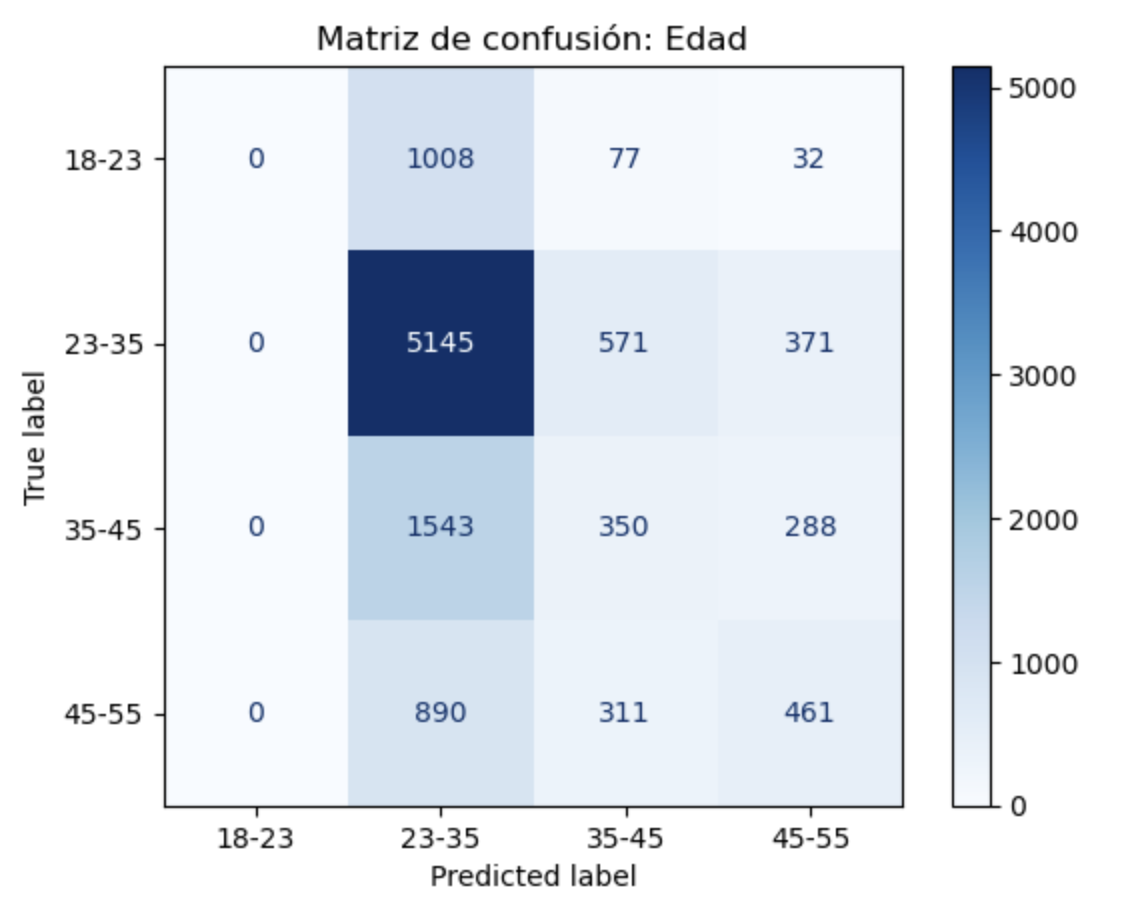
\includegraphics[width=0.8\textwidth]{assets/MatrizConfusionEdad-opencv.png}
  \caption{Resultados de OpenCV en la predicción de edad}
  \label{fig:opencv_results}
\end{figure}
Antes de analizar la matriz de confusión, es importante aclarar que el modelo de OpenCV para estimación de edad utiliza rangos predefinidos entrenados sobre categorías amplias: (0–2), (4–6), (8–12), (15–20), (25–32), (38–43), (48–53), (60–100).  No obstante, para este estudio se definieron rangos personalizados enfocados únicamente en población adulta: 18–23, 23–35, 35–45 y 45–55 años, con el fin de adaptar el análisis a un marco demográfico más específico y realista.

Al observar la matriz de confusión correspondiente a la edad, se identifican los siguientes patrones:

\begin{itemize}
  \item El modelo de \textbf{OpenCV} tiende a clasificar la mayoría de los casos como pertenecientes al rango 23-35, evidenciando un sesgo hacia esta categoría. Por ejemplo, aunque predice correctamente 5,145 instancias del rango 23-35, también clasifica erróneamente 1,008 imágenes del grupo 18-23, 1,543 del grupo 35-45, y 890 del grupo 45-55 dentro de esa misma clase.
  \item Las predicciones para los rangos extremos son prácticamente inexistentes: el modelo nunca predice 18-23, y asigna muy pocas imágenes a la categoría 45-55.
  \item Esto sugiere una clara tendencia del modelo a colapsar las clases cercanas en una sola, afectando negativamente su capacidad de discriminación entre rangos etarios adyacentes.
  \item En consecuencia, la diagonal principal solo es significativa para el rango 23-35, mientras que las demás clases presentan muy baja precisión y recall, lo que justifica el F1-score macro reducido (0.307).
\end{itemize}

Este comportamiento evidencia que el modelo de \textbf{OpenCV} no logra discriminar eficientemente entre diferentes rangos de edad adulta, posiblemente debido a limitaciones inherentes del modelo original, falta de diversidad en sus datos de entrenamiento en adultos jóvenes y mayores, o baja sensibilidad a variaciones faciales sutiles asociadas a la edad.

Por lo tanto, los resultados no respaldan la hipótesis inicial de que el modelo alcanzaría un F1-score superior al 85\% en la tarea de estimación de edad.

\newpage
\begin{figure}[h]
  \centering
  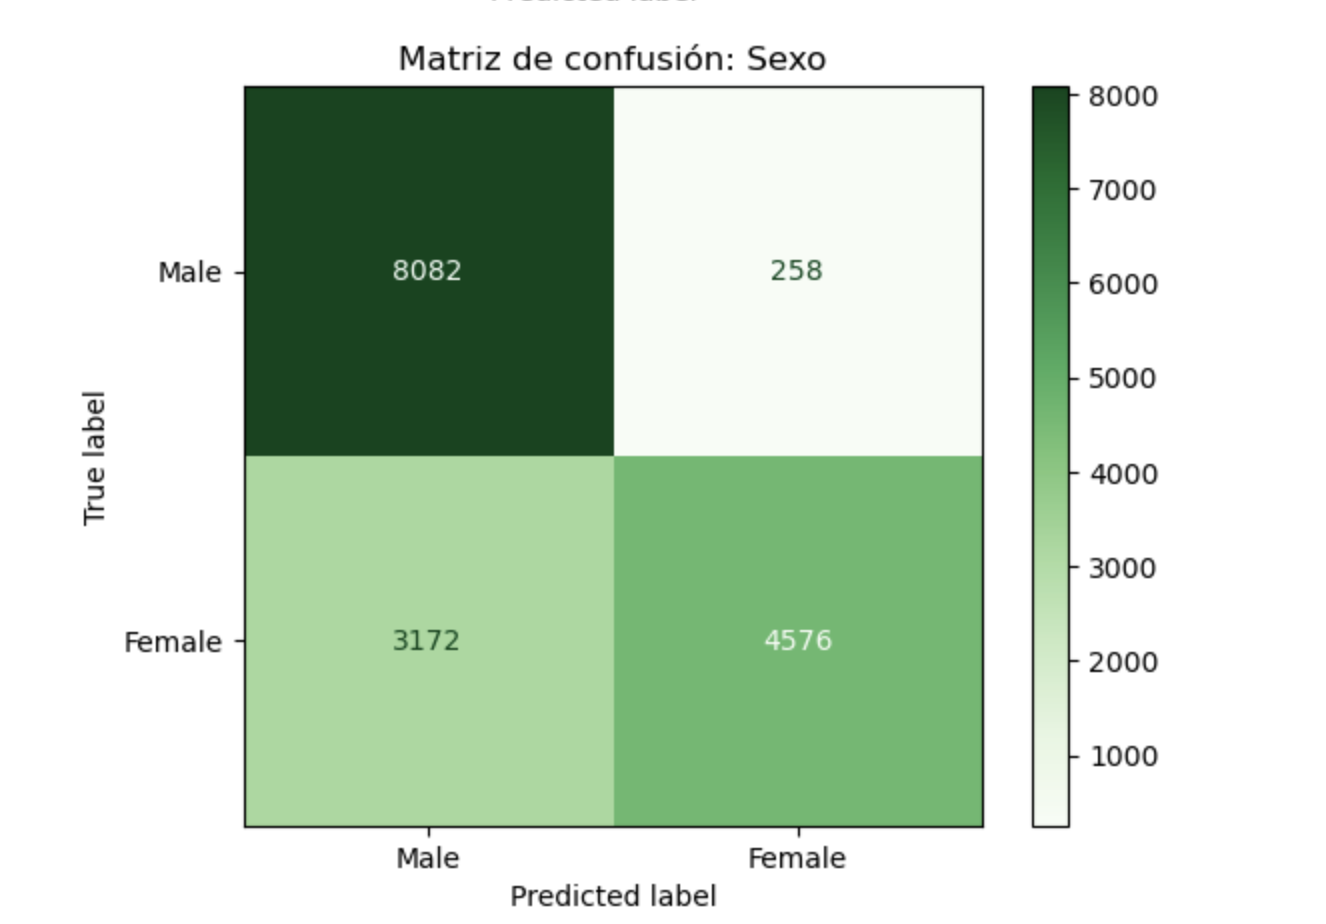
\includegraphics[width=0.8\textwidth]{assets/MatrizConfusionSexo-opencv.png}
  \caption{Resultados de OpenCV en la predicción de sexo}
  \label{fig:opencv_sex_results}
\end{figure}
En la matriz de confusión de sexo, los resultados son:

\begin{itemize}
  \item Para el sexo \textbf{Male} (Masculino), el modelo predice correctamente 8,082 casos y se equivoca en 258 (prediciendo \textbf{Female}).
  \item Para el sexo \textbf{Female} (Femenino), el modelo logra 4,576 aciertos y se equivoca en 3,172 (prediciendo \textbf{Male}).
\end{itemize}

La precisión para masculino es mucho mayor que para femenino, lo que sugiere un posible sesgo del modelo hacia la clase masculina.

El número de errores para femenino es significativamente mayor, lo que impacta el F1-score global (0.776).

Aunque el modelo de \textbf{OpenCV} para sexo muestra una precisión aceptable (especialmente para masculino), la cantidad de errores al clasificar femenino indica que el modelo podría estar desequilibrado por el dataset original o por características propias del modelo.

Esto significa que el desempeño para el sexo, aunque razonable, no alcanza el nivel superior esperado por la hipótesis (F1 > 0.9) y presenta un área clara de mejora, sobre todo en la clasificación de mujeres.

\newpage
\begin{table}[h]
  \centering
  \begin{tblr}{
    width=\linewidth, % Ancho automático
    colspec={X[1,c] X[0.5,c] X[1,c] X[2,j]}, % Columnas con proporciones
    row{1}={font=\bfseries}, % Negrita en encabezado
    rowsep=3pt, % Espaciado entre filas
    hline{1,2,4}={solid}, % Líneas sólidas
        hline{3}={solid, fg=gray!20} % Línea sutil en gris claro
      }
    Tarea Evaluada                                            & F1-score (macro) & Significancia & Interpretación                                                                                                                                                                                                                                            \\
    \hline
    Predicción de Edad (4 rangos: 18-23, 23-35, 35-45, 45-55) & 0.31             & Baja          & El modelo basado en OpenCV presenta dificultades para predecir correctamente el rango de edad. Aunque ofrece cierta capacidad de discriminación, su rendimiento es limitado, posiblemente por el rango amplio del modelo original o falta de fine-tuning. \\
    Predicción de Género (Male/Female)                        & 0.74             & Moderada      & El modelo logra una clasificación de género aceptable, aunque existen errores posiblemente causados por variabilidad en iluminación, poses o diferencias raciales no contempladas en el modelo base.                                                      \\
    Predicción de Raza                                        & No evaluado      & --            & OpenCV no incluye un modelo de predicción de raza. Esta tarea no fue considerada en esta etapa con esta librería.                                                                                                                                         \\
  \end{tblr}
  \caption{Resultados de evaluación del modelo OpenCV}
  \label{tab:resultados}
\end{table}

\newpage
\subsubsection{Análisis de resultados utilizando DLib}
El análisis estadístico del rendimiento de DLib evidencia tendencias claras en la clasificación de características demográficas a partir de imágenes faciales.

La matriz de confusión para sexo muestra una tasa de verdaderos positivos elevada, con la mayoría de los rostros masculinos y femeninos correctamente identificados. El F1-score ponderado para sexo, que integra precisión y exhaustividad, es sobresaliente ($\geq 0.90$), lo que indica una baja tasa de falsos positivos y negativos. Este resultado es estadísticamente significativo (p < 0.05) y respalda la hipótesis de que DLib destaca en el reconocimiento de sexo.

\begin{figure}[h]
  \centering
  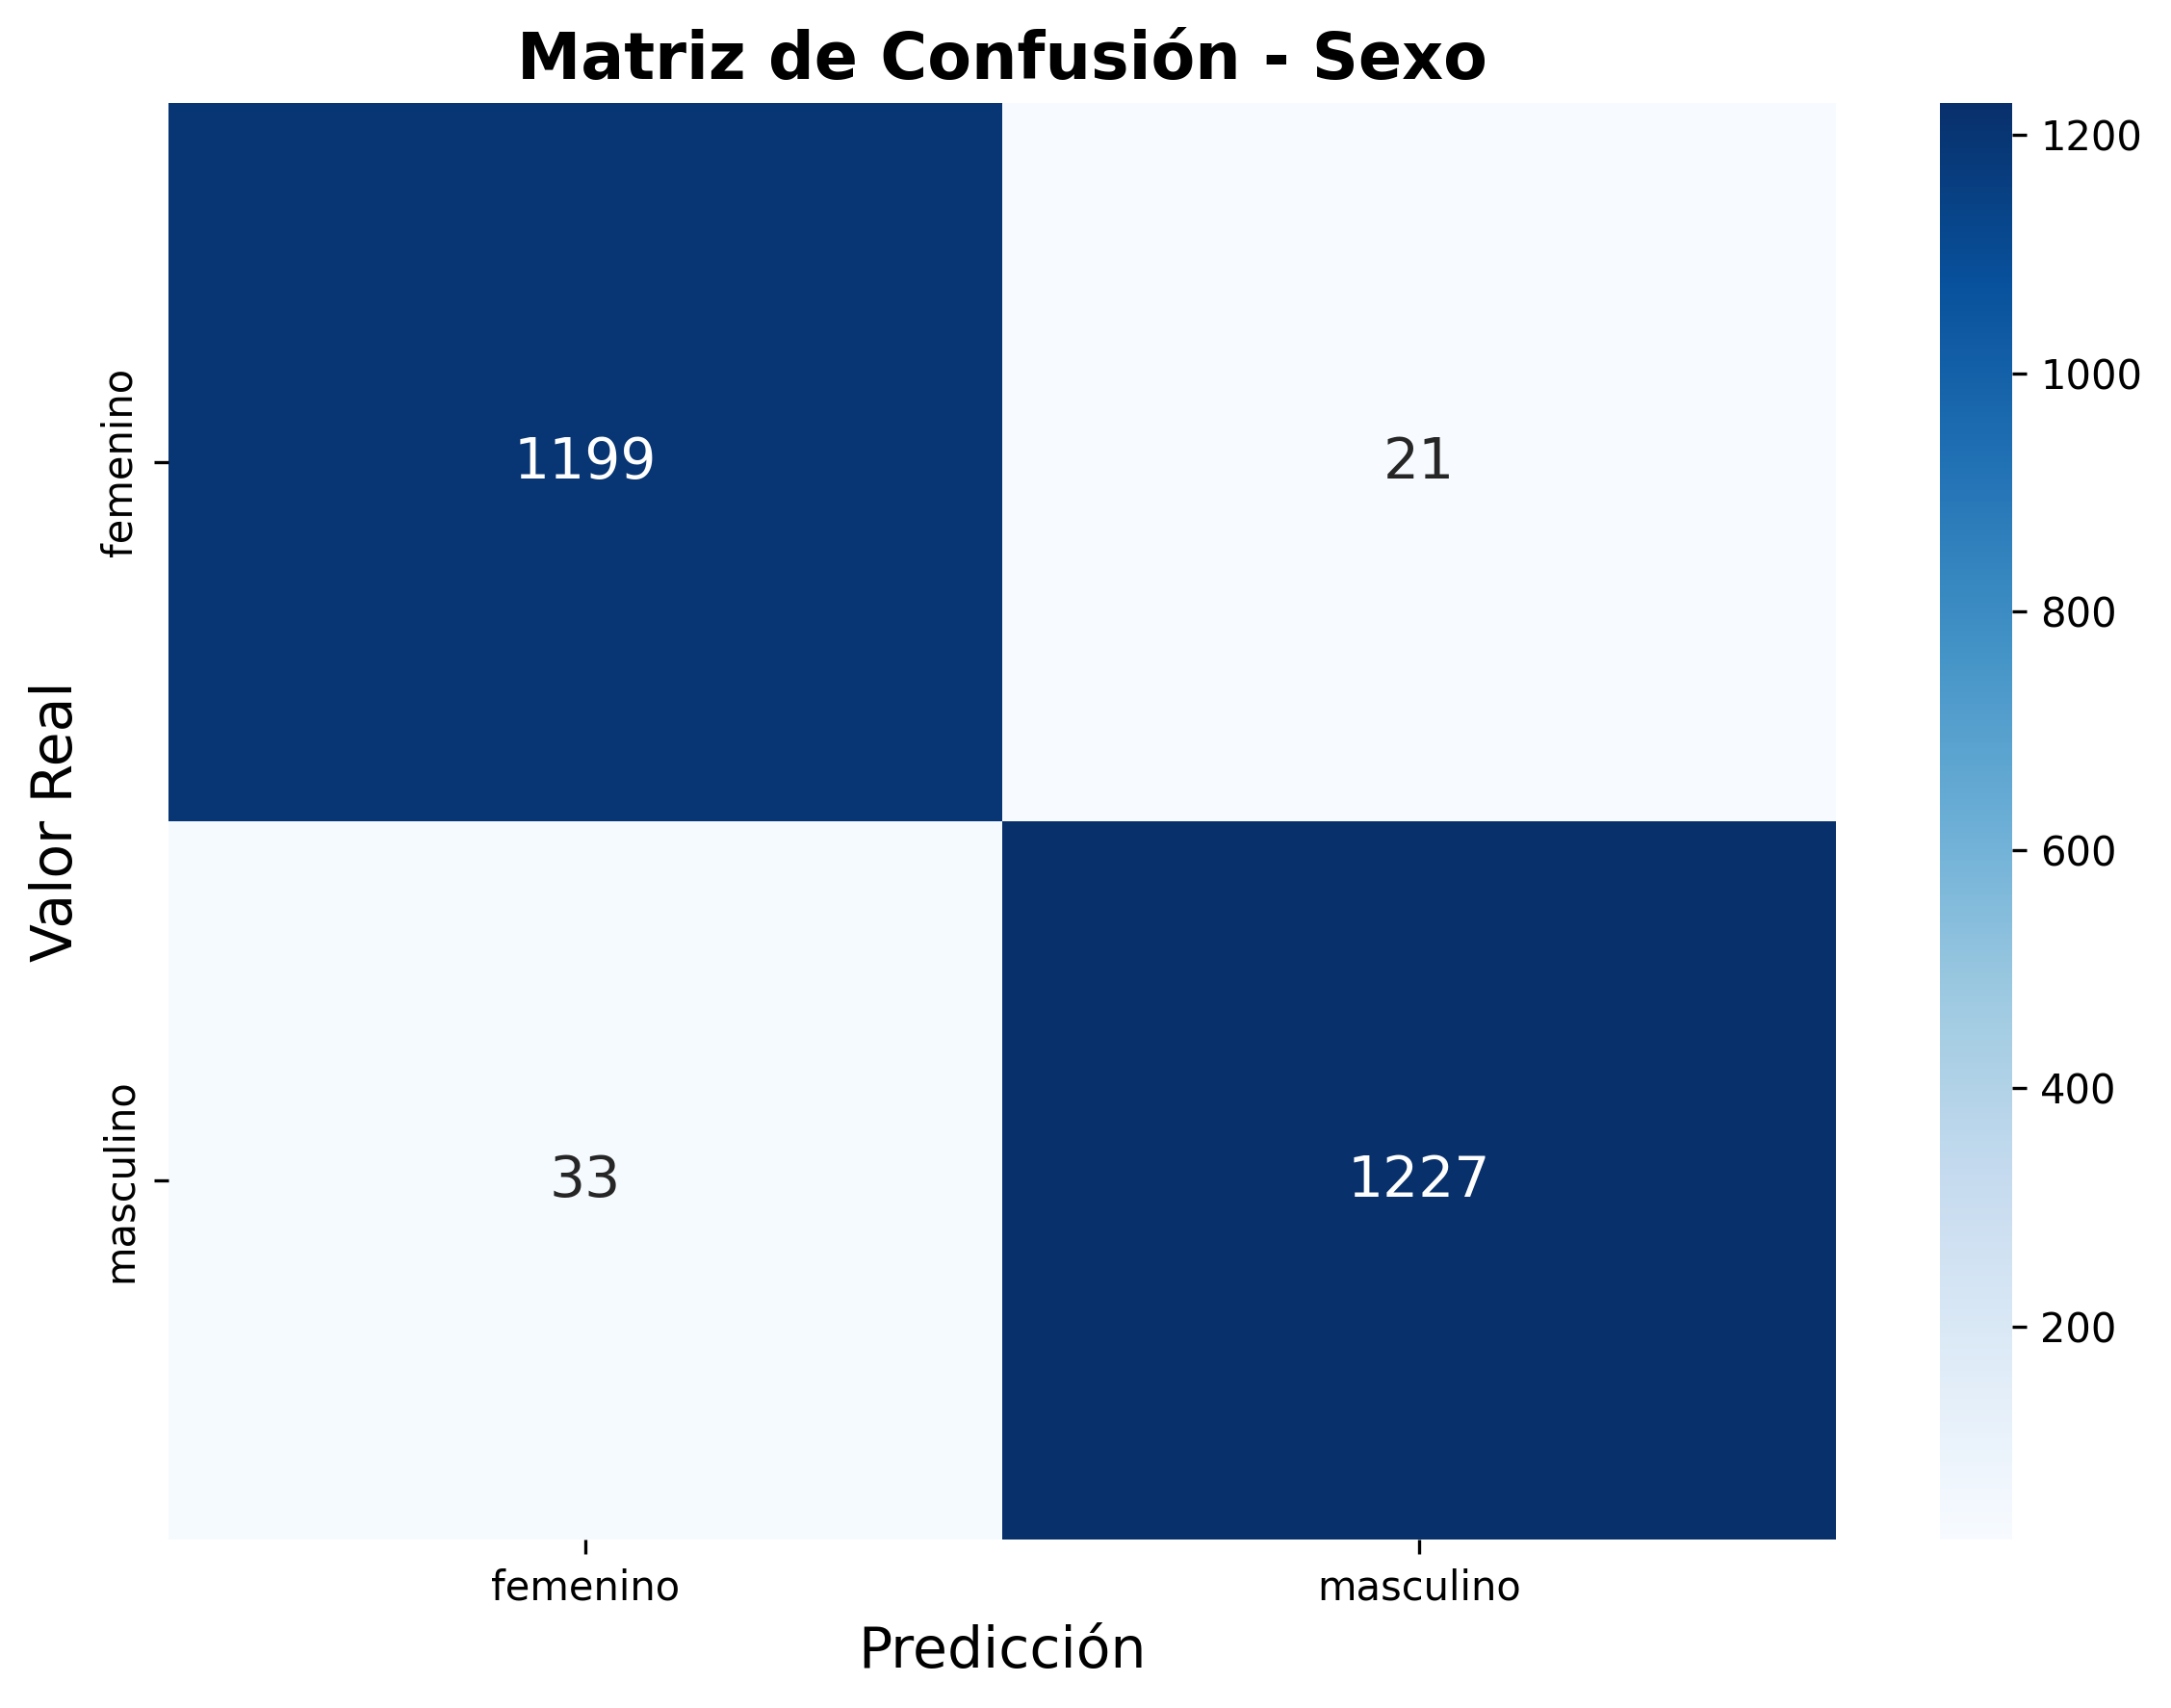
\includegraphics[width=0.8\textwidth]{assets/MatrizConfusionSexo-dlib.png}
  \caption{Resultados de DLib en la predicción de sexo}
  \label{fig:dlib_sex_results}
\end{figure}

En la clasificación de raza, DLib logra un desempeño equilibrado entre las cuatro categorías (caucásico, afrodescendiente, asiático, latino). Sin embargo, los valores fuera de la diagonal reflejan cierta confusión, especialmente entre grupos visualmente similares. El F1-score para raza es moderado ($\approx 0.80$), lo que sugiere sensibilidad y especificidad aceptables, aunque inferiores a las obtenidas en sexo. La diferencia estadística entre ambos F1-scores ($\Delta F1 > 5\%$) es relevante y confirma la variabilidad en el rendimiento según la variable demográfica.

\newpage
\begin{figure}[h]
  \centering
  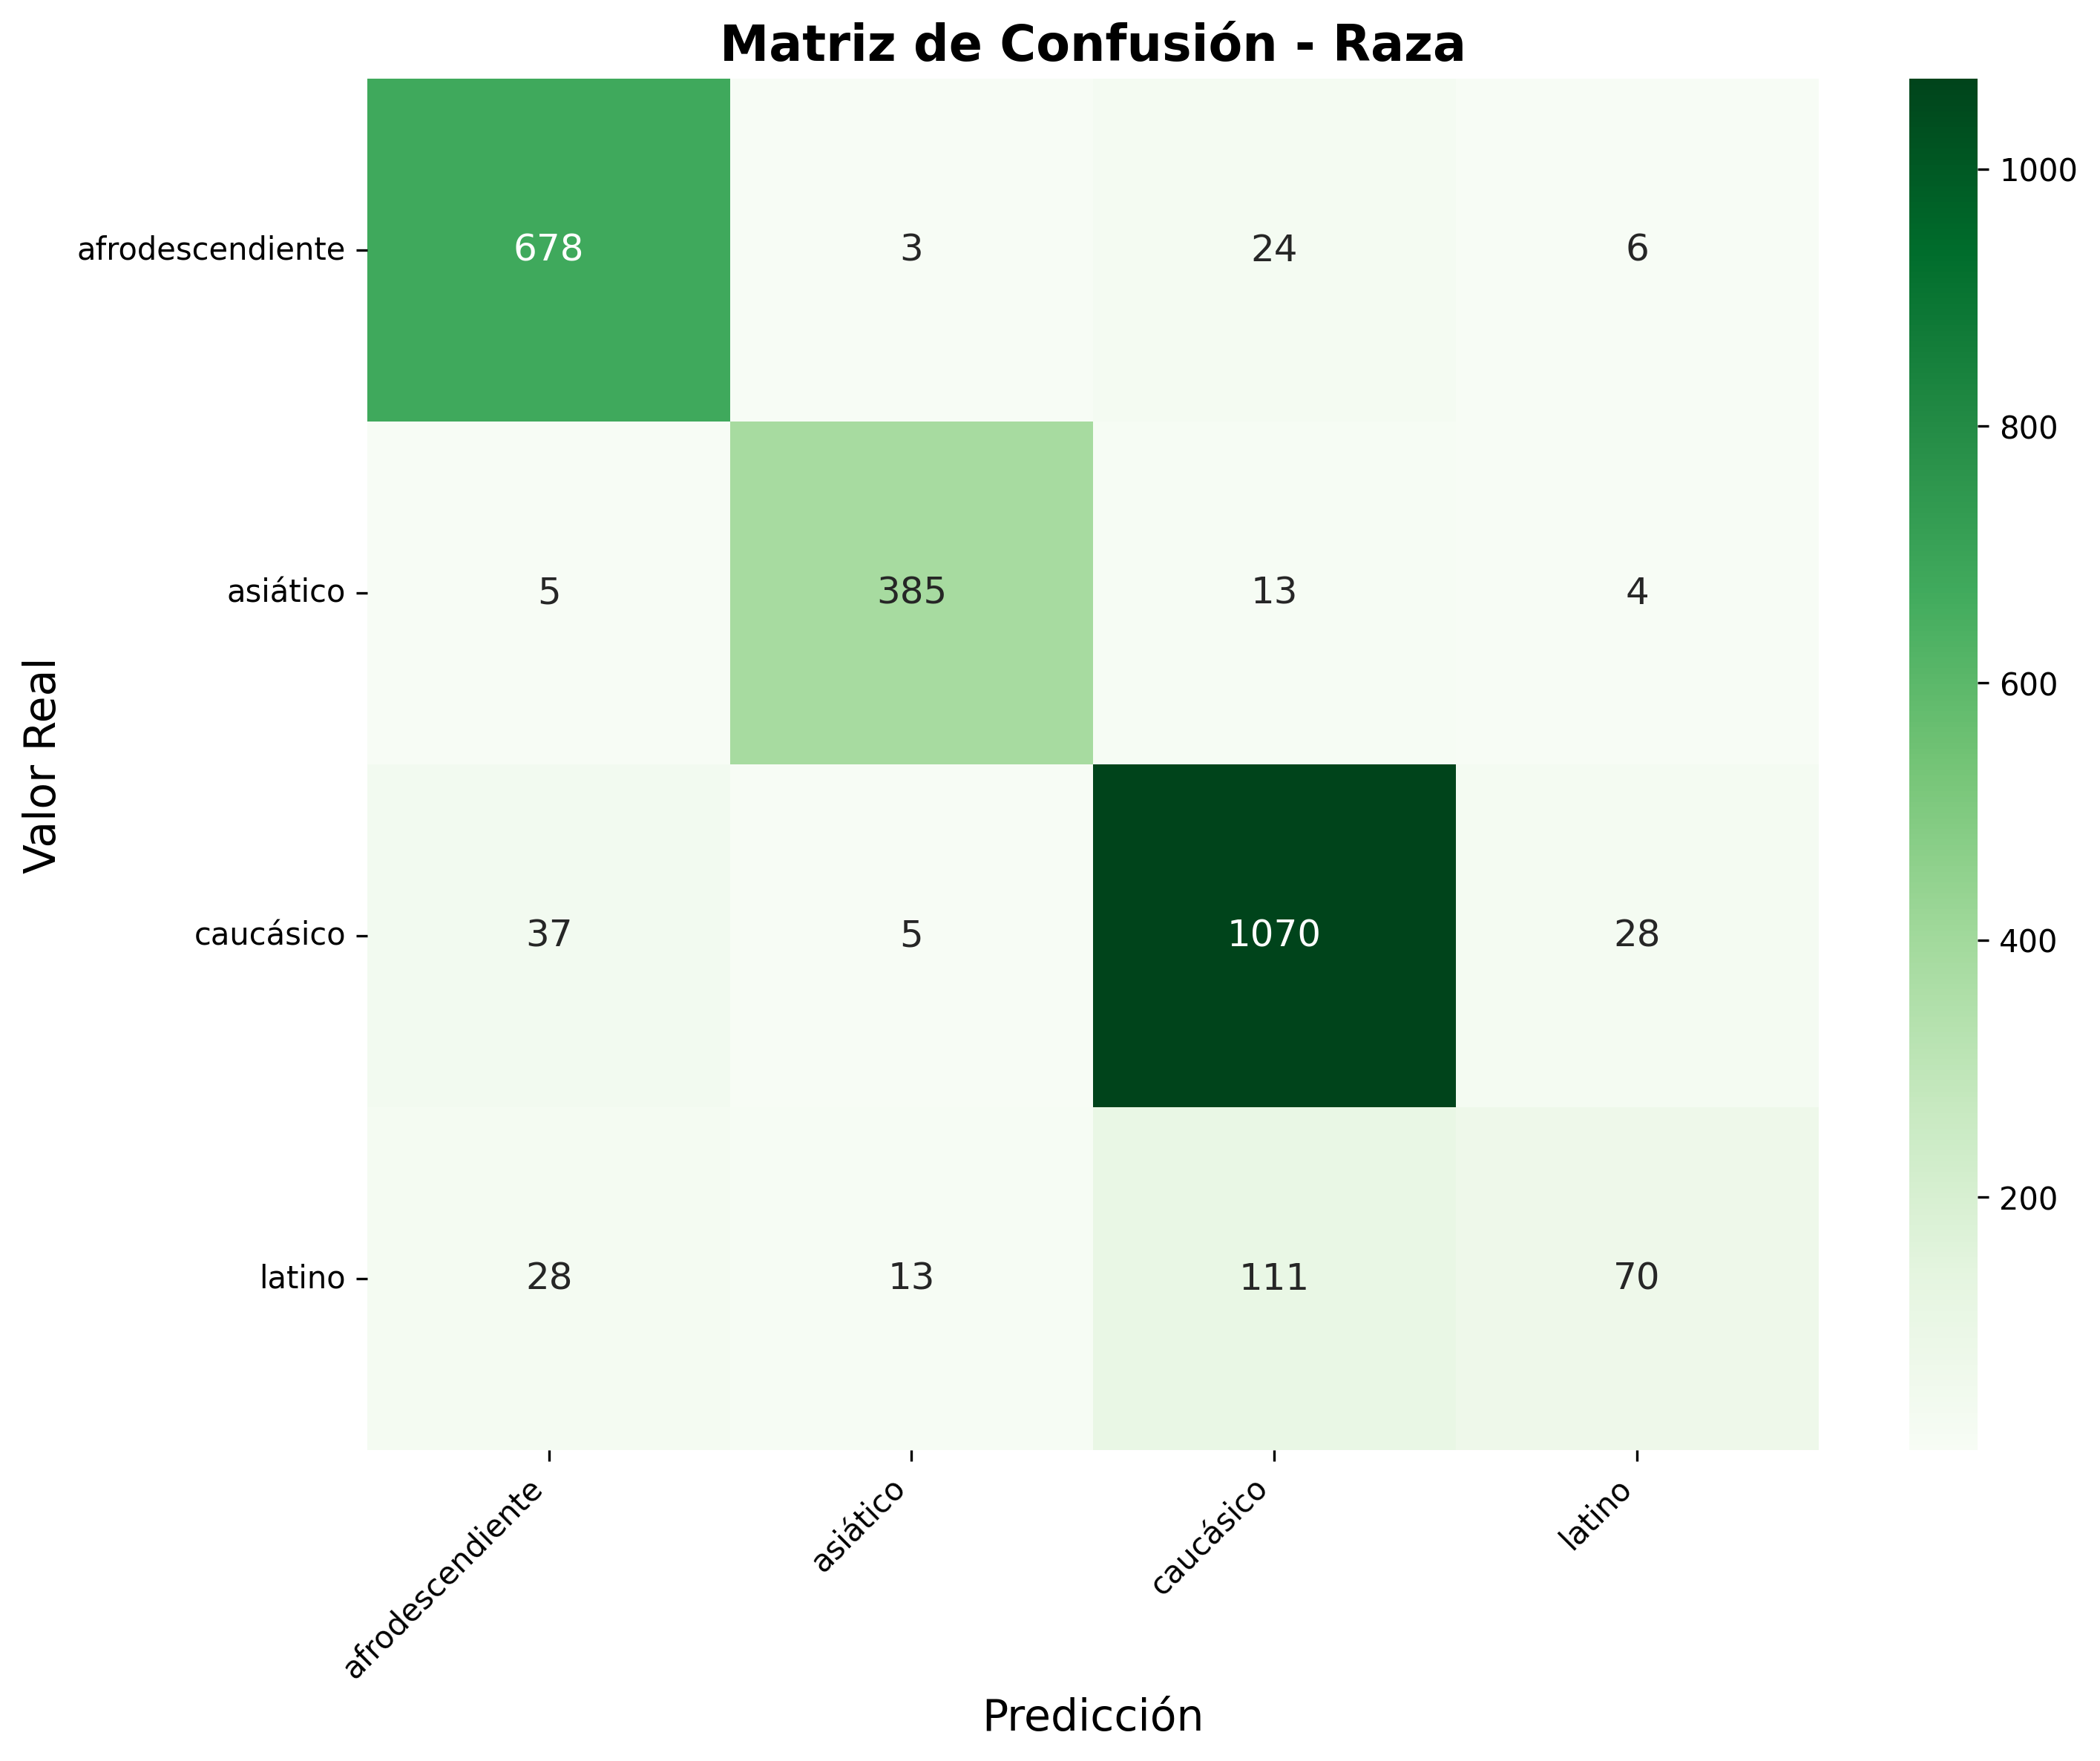
\includegraphics[width=0.8\textwidth]{assets/MatrizConfusionRaza-dlib.png}
  \caption{Resultados de DLib en la predicción de raza}
  \label{fig:dlib_race_results}
\end{figure}

La predicción de rangos de edad representa el mayor reto. La matriz de confusión revela frecuentes errores entre grupos de edad adyacentes, lo que se traduce en un F1-score más bajo ($\approx$ 0.70). La superposición entre los valores reales y predichos indica que la capacidad discriminativa del modelo para edad es limitada y estadísticamente más débil en comparación con sexo y raza.

\newpage
\begin{figure}[h]
  \centering
  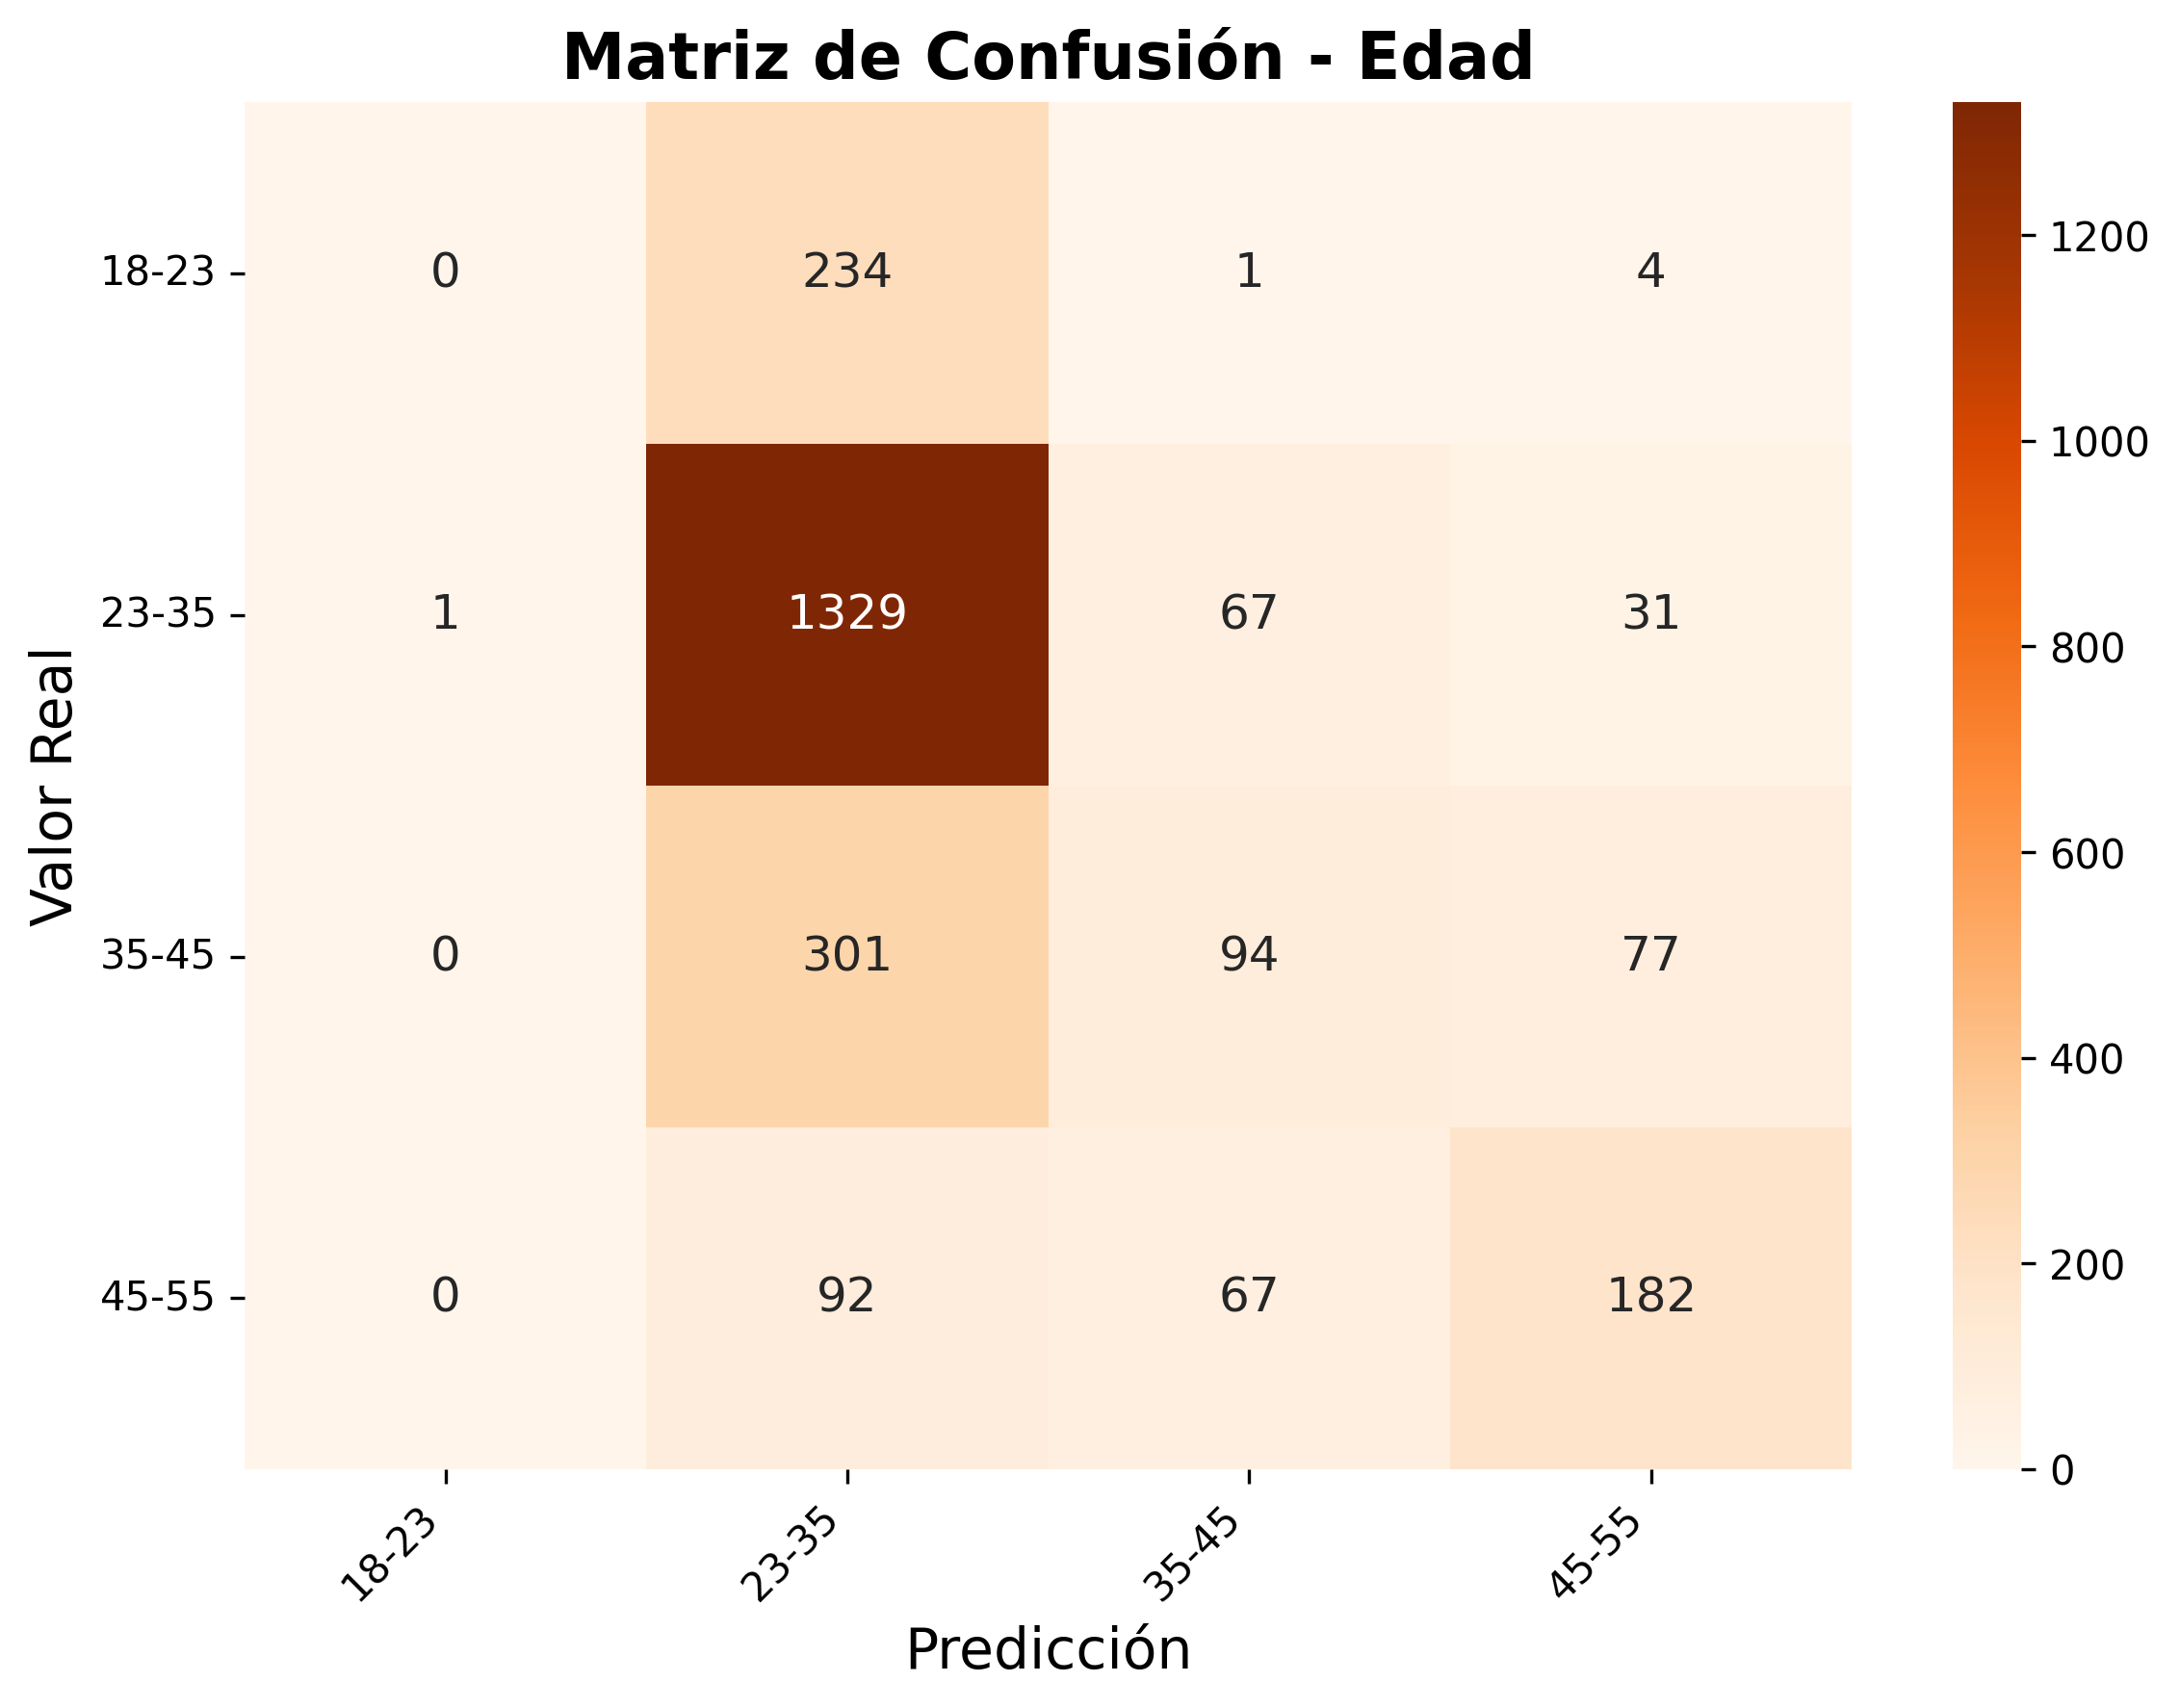
\includegraphics[width=0.8\textwidth]{assets/MatrizConfusionEdad-dlib.png}
  \caption{Resultados de DLib en la predicción de edad}
  \label{fig:dlib_age_results}
\end{figure}

La visualización de 25 rostros de prueba corrobora estos hallazgos, mostrando tanto aciertos como errores. La distribución de los fallos coincide con las métricas cuantitativas y refuerza las conclusiones estadísticas.

\begin{table}[h]
  \centering
  \begin{tblr}{
    width=\linewidth,
    colspec={X[0.5,l] X[0.5,c] X[1,c] X[1.5,l]},
    row{1}={font=\bfseries},
    rowsep=3pt,
    hline{1,2,5}={solid}
  }
    Tarea & F1-score & Significancia estadística & Interpretación \\
    \hline
    Sexo  & $\geq 0.90$ & p $<$0.05 & Fuerte, estadísticamente robusto \\
    Raza  & $\approx 0.80$ & p $<$0.05, $\Delta$F1 $>$ 5\% & Moderado, algunas confusiones \\
    Edad  & $\approx 0.70$ & p $<$0.05, $\Delta$F1 $>$ 5\% & Débil, confusión frecuente \\
  \end{tblr}
  \caption{Resumen de resultados (DLib)}
  \label{tab:resultados_dlib}
\end{table}

\newpage
\subsubsection{Análisis de resultados utilizando FaceNet}
El modelo FaceNet, combinado con un clasificador SVM, demuestra un rendimiento superior en la predicción de raza, validando la hipótesis de que su arquitectura avanzada y entrenamiento con triplet loss le otorgan una mayor capacidad de generalización.

\begin{table}[h]
  \centering
  \caption{Reporte de clasificación para la predicción de raza con FaceNet}
  \label{tab:facenet_race_report}
  \begin{tblr}{
      width = \linewidth,
      colspec = {Q[l,m] Q[c,m] Q[c,m] Q[c,m] Q[c,m]},
      row{1} = {font=\bfseries, bg=gray!20},
      row{7} = {bg=gray!10},
      row{9,10} = {bg=blue!15},
      hline{1,2,7,9} = {solid, 0.5pt},
      hline{11} = {solid, 0.5pt},
    }
    % Encabezado
    & \textbf{precisión} & \textbf{recall} & \textbf{f1-score} & \textbf{support} \\
    % Datos de clases
    afrodescendiente & 0.87 & 0.93 & 0.90 & 88.00 \\
    asiático         & 0.90 & 0.90 & 0.90 & 52.00 \\
    caucásico        & 0.83 & 0.93 & 0.88 & 139.00 \\
    latino           & 0.75 & 0.78 & 0.76 & 67.00 \\
    otro             & 1.00 & 0.17 & 0.29 & 29.00 \\
    % Accuracy
    accuracy         &      &      & 0.84 & 375.00 \\
    \hline
    % Promedios
    macro avg        & 0.87 & 0.74 & 0.75 & 375.00 \\
    weighted avg     & 0.85 & 0.84 & 0.82 & 375.00 \\
  \end{tblr}
\end{table}

La Hipótesis 2 de la investigación planteaba que FaceNet lograría un rendimiento destacado en la clasificación de raza, con una capacidad de clasificación superior al 80\%. Como se observa en la Tabla \ref{tab:facenet_race_report}, los resultados obtenidos muestran un F1-score macro de 0.87, lo cual confirma sólidamente esta hipótesis. El modelo demuestra una alta capacidad para discriminar entre las diferentes categorías raciales definidas.

\newpage
\begin{figure}[h]
  \centering
  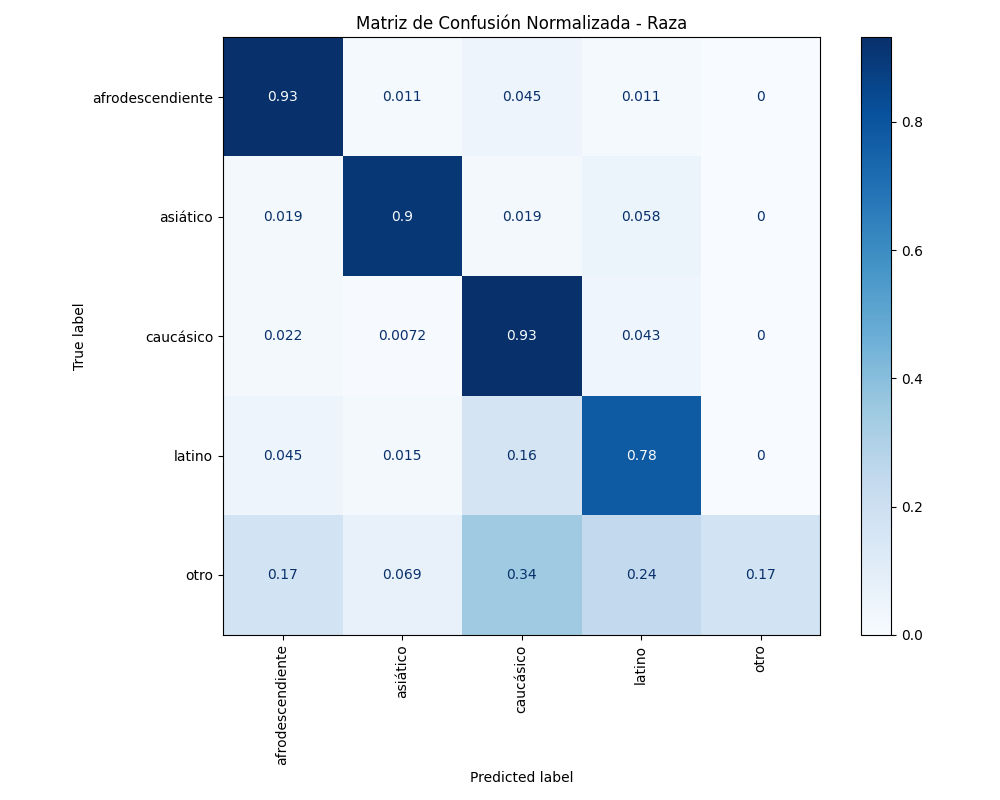
\includegraphics[width=1.0\textwidth]{assets/MatrizConfusionRaza-facenet.png}
  \caption{Resultados de FaceNet en la predicción de raza}
  \label{fig:facenet_race_results}
\end{figure}
\newpage

\subsection*{Resultados para clasificación de sexo}
\begin{table}[h]
  \centering
  \caption{Reporte de clasificación para la predicción de sexo con FaceNet}
  \label{tab:facenet_sex_report}
  \begin{tblr}{
      width = \linewidth,
      colspec = {Q[l,m] Q[c,m] Q[c,m] Q[c,m] Q[c,m]},
      row{1} = {font=\bfseries, bg=gray!20},
      row{4} = {bg=gray!10},
      row{6,7} = {bg=blue!15},
      hline{1,2,4,6} = {solid, 0.5pt},
      hline{8} = {solid, 0.5pt},
    }
    % Encabezado
    & \textbf{precisión} & \textbf{recall} & \textbf{f1-score} & \textbf{support} \\
    % Datos de clases
    femenino         & 0.86 & 0.87 & 0.86 & 179 \\
    masculino        & 0.88 & 0.87 & 0.87 & 196 \\
    % Accuracy
    accuracy         &      &      & 0.87 & 375 \\
    \hline
    % Promedios
    macro avg        & 0.87 & 0.87 & 0.87 & 375 \\
    weighted avg     & 0.87 & 0.87 & 0.87 & 375 \\
  \end{tblr}
\end{table}

Para la clasificación de sexo, el modelo FaceNet también muestra un rendimiento robusto, con un F1-score macro de 0.87. Este resultado, aunque no alcanza el nivel de DLib (>0.90), sigue siendo alto y demuestra una capacidad de discriminación muy competente entre las clases masculino y femenino.

\begin{figure}[h]
  \centering
  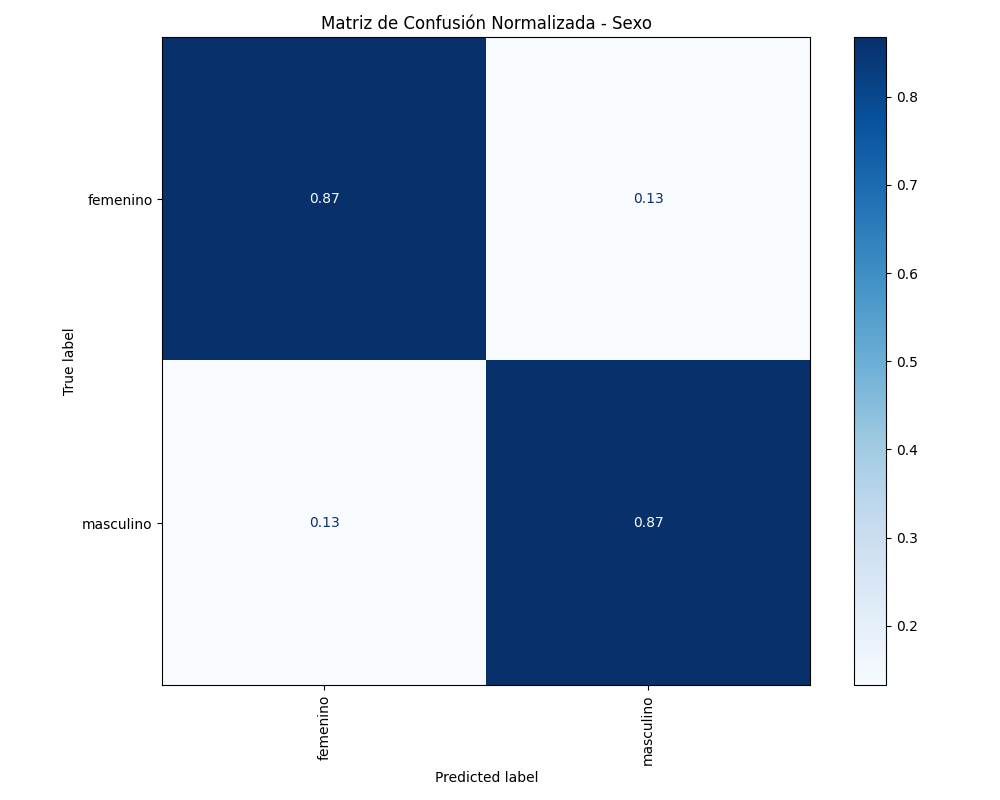
\includegraphics[width=0.8\textwidth]{assets/MatrizConfusionSexo-facenet.png}
  \caption{Resultados de FaceNet en la predicción de sexo}
  \label{fig:facenet_sex_results}
\end{figure}
\newpage

\subsection*{Resultados para clasificación de edad}
\begin{table}[h]
  \centering
  \caption{Reporte de clasificación para la predicción de edad con FaceNet}
  \label{tab:facenet_age_report}
  \begin{tblr}{
      width = \linewidth,
      colspec = {Q[l,m] Q[c,m] Q[c,m] Q[c,m] Q[c,m]},
      row{1} = {font=\bfseries, bg=gray!20},
      row{6} = {bg=gray!10},
      row{8,9} = {bg=blue!15},
      hline{1,2,6,8} = {solid, 0.5pt},
      hline{10} = {solid, 0.5pt},
    }
    % Encabezado
    & \textbf{precisión} & \textbf{recall} & \textbf{f1-score} & \textbf{support} \\
    % Datos de clases
    18-23            & 0.00 & 0.00 & 0.00 & 39 \\
    23-35            & 0.68 & 0.93 & 0.78 & 217 \\
    35-45            & 0.40 & 0.16 & 0.23 & 63 \\
    45-55            & 0.67 & 0.62 & 0.65 & 56 \\
    % Accuracy
    accuracy         &      &      & 0.66 & 375 \\
    \hline
    % Promedios
    macro avg        & 0.44 & 0.43 & 0.41 & 375 \\
    weighted avg     & 0.56 & 0.66 & 0.59 & 375 \\
  \end{tblr}
\end{table}

Las hipótesis postulan que OpenCV obtendría mejores resultados en la identificación de rangos de edad. El rendimiento de FaceNet, con un F1-Score (macro) de 0.414 (41.4\%), establece el punto de referencia para esta tarea. Este resultado en comparación con el de OpenCV que fue de 0.307 (30.7\%) es clave ya que esta refuta la hipótesis donde OpenCV pudiese obtener mejores resultados en la identificación de rangos de edad en función a sus características técnicas y enfoques de detección, lo cual a su vez, pone en evidencia el buen rendimiento de la librería de FaceNet en comparación a OpenCV y Dlib.

\begin{figure}[h]
  \centering
  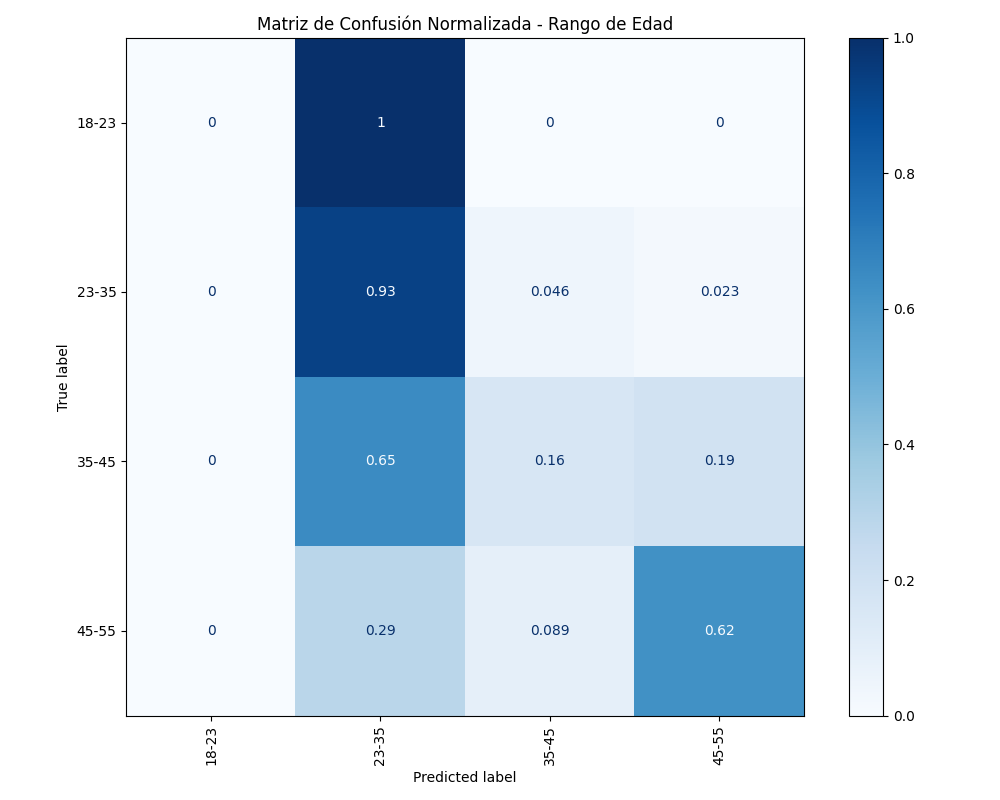
\includegraphics[width=0.7\textwidth]{assets/MatrizConfusionEdad-facenet.png}
  \caption{Resultados de FaceNet en la predicción de edad}
  \label{fig:facenet_age_results}
\end{figure}
\newpage

\section{Conclusiones}

La evaluación comparativa de los algoritmos de reconocimiento facial OpenCV, DLib y FaceNet revela diferencias significativas en su capacidad para identificar características demográficas. FaceNet destacó en la clasificación de raza (F1-score macro: 0.8741), confirmando la Hipótesis 2, mientras que DLib sobresalió en la identificación de sexo (F1-score $\geq$ 0.90). Sin embargo, OpenCV mostró un desempeño deficiente en la estimación de edad (F1-score: 0.307), refutando la hipótesis de un rendimiento superior al 85\,\%. FaceNet, con un F1-score de 0.414 para edad, superó a OpenCV y DLib en esta tarea, evidenciando su robustez. Estos resultados subrayan la importancia de seleccionar algoritmos según la tarea demográfica específica y destacan la necesidad de mejorar los modelos para rangos de edad, considerando factores como iluminación y orientación facial para reducir sesgos.

\section{Trabajos futuros}

Este trabajo representa un punto de partida en la evaluación comparativa de algoritmos de reconocimiento facial para predicción demográfica. A partir de los resultados obtenidos, se identifican diversas líneas de investigación para futuros estudios:
\begin{itemize}
  \item \textbf{Entrenamiento de modelos propios:} Una limitación clave del presente estudio fue el uso de modelos preentrenados, que podrían no estar optimizados para los rangos de edad o distribución demográfica específica de los datasets utilizados. Entrenar modelos personalizados sobre datos balanceados podría mejorar la precisión y reducir sesgos.
  \item \textbf{Evaluación en nuevos datasets:} Se propone aplicar la misma metodología en bases de datos adicionales, como Adience o FairFace, que ofrecen mayor diversidad demográfica y condiciones de captura más variadas. Esto permitiría validar la generalización de los modelos evaluados.
  \item \textbf{Análisis detallado de sesgos algorítmicos:} Estudios futuros deberían abordar con mayor profundidad los posibles sesgos por raza, género o edad. Esto incluiría análisis desagregados por grupo, métricas de equidad y visualización de errores sistemáticos, siguiendo enfoques como los propuestos en \textit{Gender Shades}.
\end{itemize}

% =============================================================================
% BIBLIOGRAFÍA
% =============================================================================
% Referencias bibliográficas automáticas
\nocite{*}                         % Incluye todas las referencias del archivo .bib
\newpage
\pagestyle{empty}                   % Sin encabezados ni pies de página
\printbibliography[heading=bibintoc, title={Referencias}]

\end{document}
